% Exam document template for the informatics course given
% at HES-SO Valais // Wallis for the ISC programme
% @author Pierre-André Mudry, pierre-andre.mudry@hevs.ch
% @version 1.3
% @date September 2009
% @revision October 2010
% @revision August 2023
 
\newcommand{\path}{../../texcommon/}

% Allows flags at compile time
\ifdefined\withanswers
	\documentclass[10pt, a4paper, answers, addpoints]{\path exam}
\else
	\documentclass[10pt, a4paper, noanswers, addpoints]{\path exam}
\fi

%%%%%%%%%%%%%%%%%%%%%%%%%
% Change according to the exam type %%
%%%%%%%%%%%%%%%%%%%%%%%%%
%\def\thetitle{Test annuel -- Jahrespr\"{u}fung} 
%\def\thetitle{Test semestriel -- Semesterp\"{u}fung}
\def\thetitle{Test interm\'{e}diaire}
\def\exam{}
\def\examMonth{Octobre 2022}
\def\examDate{27.10.2022} 
\def\rev{Rev 1.04$\omega$} 

\input{\path options}
 
\usepackage{float}
\usepackage{fontawesome}
\usepackage{gensymb}

%%%%%%%%%%%%%%%%%%%%%%%%%
% Uncomment this for the draft versions %%
%%%%%%%%%%%%%%%%%%%%%%%%%
%\def\confidential{}

%%%%%%%%%%%%%%%%%%%%%%%%%
% Configure exam class %%
%%%%%%%%%%%%%%%%%%%%%%%%%
% Header and footer configuration, special for the exam
\noheadrule
\runningheadrule
\header
	{\makebox[8cm]{\large{Nom :}\enspace\dotfill}\\\vspace{0.4cm}\makebox[8cm]{\large{Prénom :}\enspace\dotfill}}
	{}	
	{}{}{}
	\runningheader{\oddeven{}{\small{\examDate{}}}}
	{}
	{\oddeven{\textsc{\thetitle{}}}}

\footrule

\firstpagefooter{\small{Dr P.-A. Mudry}} {\small{\examMonth}} {\small{Page \thepage/\numpages}}

\runningfooter{\oddeven{\small{Page \thepage/\numpages}}{\includegraphics[width=2.2cm]{\path logo.pdf}}}{\iflastpage{The end}{}}{\oddeven{{\includegraphics[width=2.2cm]{\path logo.pdf}}}{\small{Page \thepage/\numpages}}}

\setlength\answerlinelength{3 cm}
\setlength\headsep{0.7cm}

\marginpointname{ Pt}
%\pointsinrightmargin
\pointsinmargin
\bracketedpoints
\extrawidth{-2mm}
\extraheadheight[0.5cm]{-0.2cm}
\extrafootheight{-5mm}
\cvbpword{Bonus}

% Format for the questions
\qformat{\Large{\textbf{Question \thequestion{} -- \thequestiontitle}} (\totalpoints \ points)\hfill}

\marginbonuspointname{ \emph{Bo}}

%%%%%%%%%%%%%%%
% Here we go %%
%%%%%%%%%%%%%%%
\begin{document}

\vspace*{1.5cm} 
\hrule
% Title  
{
	\huge
	\begin{center}
		\textsc{\thetitle}\\
		\ifprintanswers{}
		\Large{SOLUTION}\\
		\large \textit {101.1 -- Programmation impérative}\\
		\else
		\Large \textit{101.1 -- Programmation impérative}\\
		\fi
	\end{center}
}
\hrule
\vspace{2.5cm}
 
% Create the box for the directions
\titlebox{
	{\large{\textbf{Consigne : }}}\\

	Lisez attentivement la donnée et répondez de manière \textbf{lisible} aux questions. Vous avez droit pour cet examen à un aide-mémoire de 1 pages (1 feuille recto). Aucun moyen électronique n'est permis.\\
	
	Un conseil : ne restez pas bloqués sur une question. Répondez tout d'abord aux questions avec lesquelles vous êtes à l'aise et revenez ensuite aux questions posant problème. Le barème indiqué est indicatif. 
	\vspace{5mm}

	\begin{center} 
		\combinedgradetable[v][questions]\\
		\vspace{3mm}
		\small{This exam has \numquestions\ questions, for a total of \numpoints\ points.}
	\end{center}
	\vspace{5mm}
}

%\vspace{1mm}
%\hrule 
%\vspace{3mm}
\begin{center}\tiny{\rev}\end{center}

\begin{tikzpicture}[remember picture,overlay]
	\node[anchor=north east,inner sep=0pt] at ($(current page.north east)+(-1.2cm,-0.5cm)$) {
		\includegraphics[width=8.5cm]{\path isc_logo_inline.pdf}
	};
\end{tikzpicture}


%\leerseite{}
\newpage

%%%%%%%%%%%%%%%%
% Let's start asking things
%%%%%%%%%%%%%%%%

\begin{questions}
%%%%%%%%%%%%%%%%%%%%%%%%%%%%%%%%%%%%%%%%%%%%
\titledquestion{Short questions}
%%%%%%%%%%%%%%%%%%%%%%%%%%%%%%%%%%%%%%%%%%%%

Cette question est séparée en plusieurs exercices indépendants. Le nombre de point pour chaque exercice est indiqué dans la marge.

\begin{parts}
%%%%%%%%%%%%%%%%%%%%%%%%%%
\part[4]
%%%%%%%%%%%%%%%%%%%%%%%%%%
Soient les déclarations suivantes:

\begin{scala}
	val foo : Int = 0xBABA
	val foobar : Float = 3.825f
	val baz : String = "y"
\end{scala}

Les expressions suivantes sont correctes. Donnez le \textbf{type} et la \textbf{valeur} des expressions suivantes.

\begin{subparts}
	\subpart\begin{verbatim}(foobar + - foobar).toByte\end{verbatim} \answerline[Byte, 0]
	\subpart\begin{verbatim}(foo & 0xFF0).toHexString\end{verbatim} \answerline[String, "ab0"]
	\subpart\begin{verbatim}(((foo >> 4) << 4) | 0xE).toHexString\end{verbatim} \answerline[String, "babe"]
	\subpart\begin{verbatim}(foo^foo).toShort\end{verbatim} \answerline[Short, 0]
	\subpart\begin{verbatim}((foobar * 100).toInt / 100.0f)\end{verbatim} \answerline[Float, 3.82f]
	\subpart\begin{verbatim}if(foo < 0xFFFF) 'a' else 'b'\end{verbatim} \answerline[Char, 'a']
	\subpart\begin{verbatim}if(true) '1' + baz else baz + '1'\end{verbatim} \answerline[String, "1y"]
	\subpart\begin{verbatim}baz + ('d' + 1.9).toChar + ('t'-1).toChar\end{verbatim} \answerline[String, "yes"]

\end{subparts}

%%%%%%%%%%%%%%%%%%%%%%%%%%
\part[1]
%%%%%%%%%%%%%%%%%%%%%%%%%%
Quel est le contenu de \texttt{r} après l'exécution du code ci-dessous :

\begin{scala}
	val s: String = "TikTok"
	val r: String = StringUtils.charAt(s, StringUtils.length(s)-2) +
	"" + StringUtils.charAt(s, 2)
\end{scala}

\begin{solutionordottedlines}[1cm]
	"ok"
\end{solutionordottedlines}

%%%%%%%%%%%%%%%%%%%%%%%%%%
\part[1]
%%%%%%%%%%%%%%%%%%%%%%%%%%
Soit le code suivant :

\begin{scala}
	val a : Boolean = ...
	val b : Boolean = a || !a
\end{scala}

Quelle est la valeur de \texttt{b} ?
\begin{oneparcheckboxes}
	\choice Elle dépend du contenu de \texttt{a}
	\CorrectChoice \texttt{true}
	\choice \texttt{false}
\end{oneparcheckboxes}

%%%%%%%%%%%%%%%%%%%%%%%%%%
\bonuspart[2]
%%%%%%%%%%%%%%%%%%%%%%%%%%
Écrivez le code (sans fonction) permettant d'écrire tous les multiples de 79 plus grands que 1 et plus petits que 1000 sur la console.

\begin{solutionordottedlines}[\fill]
	\begin{scala}
		for (i: Int <- 1 until 1000; if i % 79 == 0)
			println(i)
	\end{scala}
\end{solutionordottedlines}

\newpage

%%%%%%%%%%%%%%%%%%%%%%%%%%
\part[4]
%%%%%%%%%%%%%%%%%%%%%%%%%%
Vrai ou faux ?
~\\
\begintruefalse{}
\truefalse{
	\texttt{(255+1).toByte == (0xFFFF+1).toShort}
}{true}

\truefalse{
	Un générateur de séquence peut générer des \texttt{Double}
}{false}

\truefalse{
	\texttt{0 to 10} est une séquence plus longue que \texttt{1 until 11}
}{true}

\truefalse{
	\textbackslash~est le caractère d'échappement
}{true}

\truefalse{
	Un programme qui compile fonctionne toujours correctement
}{false}

\truefalse{
	Le compilateur détecte les erreurs de type
}{true}

\truefalse{
	\texttt{println()} est une fonction qui retourne un \texttt{String}
}{false}

\truefalse{
	Dans l'expression \texttt{if(foo) a else b}, \texttt{a} et \texttt{b} doivent être de même type
}{false}

\vspace{1cm}

\end{parts}

%%%%%%%%%%%%%%%%%%%%%%%%%
\titledquestion{Loops analysis}[8]
%%%%%%%%%%%%%%%%%%%%%%%%%
Que vont afficher \textbf{exactement} les boucles suivantes sur la console ?

\begin{parts}
	\part
	\qquad
	\begin{minipage}{8cm}
		\begin{scala}
			var foo: Int = 3
			var bar: Int = 8
			var i : Int = 8

			do {
				bar -= bar / (i>>1)
				foo += 1 & 0
				println(bar + foo + 1)
			} while (foo + 1 < bar)
		\end{scala}
	\end{minipage}
	\quad
	\quad
	\begin{minipage}{5cm}
		Solution:
		\begin{solution}[3.5cm]
			\begin{verbatim}
10
9
8
			\end{verbatim}
		\end{solution}
	\end{minipage}

	\vspace{7mm}

	\part
	\qquad
	\begin{minipage}{8cm}
		\begin{scala}
			var j = 6
			var i = 0
			while (i != j) {
				print(i + " " + j + " * ")
				i += 1
				j -= 1
			}
		\end{scala}
	\end{minipage}
	\quad
	\quad
	\begin{minipage}{5cm}
		Solution:
		\begin{solution}[3.5cm]
			\begin{verbatim}
0 6 * 1 5 * 2 4 *
			\end{verbatim}
		\end{solution}
	\end{minipage}

	\part	
	\qquad	
	\begin{minipage}{8cm}
		\begin{scala}
			var a: Int = 0xf0
			var t: String = ""
			while (a != 0) {
			  t = (if (a % 2 == 0) '0' else '1') + t
			  a /= 2
			}
			print(t)
		\end{scala}
	\end{minipage}
	\quad
	\quad
	\begin{minipage}{5cm}
		Solution:
		\begin{solution}[3.5cm]
			\begin{verbatim} 
11110000
			\end{verbatim}
		\end{solution}
	\end{minipage}

	\part
	\qquad
	\begin{minipage}{8cm}
		\begin{scala}
			// println(5)
			for (i: Int <- 3 to 7){
				print(s"${i-1*2/3} ")
			}
		\end{scala}
	\end{minipage}
	\quad
	\quad
	\begin{minipage}{5cm}
		Solution:
		\begin{solution}[3.5cm]
			\begin{verbatim}
3 4 5 6 7
			\end{verbatim}
		\end{solution}
	\end{minipage}

\end{parts}

%%%%%%%%%%%%%%%%
%%% QUESTION %%%
%%%%%%%%%%%%%%%%%%%%%%%%%%%%%%%%%%%%%%%%%%%%%%%%%%%%%%%%%%%%%%%%%%%%%%%%%%%%%%%%
\titledquestion{EBNF grammars}
%%%%%%%%%%%%%%%%%%%%%%%%%%%%%%%%%%%%%%%%%%%%%%%%%%%%%%%%%%%%%%%%%%%%%%%%%%%%%%%%

\begin{parts}

	\part
	Soit la grammaire suivante pour \texttt{exp}

	\begin{verbatim_lst}
		factor ::= 'x' | 'y' | 'z' | parexpr
		parexpr ::= '(' exp ')'
		op ::= '+' | '-'
		exp ::= (factor op exp) | factor
	\end{verbatim_lst}

	\begin{subparts}

		\subpart[1]
		Donnez une production valide la plus courte possible pour \texttt{exp}.
		\begin{solutionordottedlines}[1cm]
			x ou alors y ou alors z
		\end{solutionordottedlines}

		\subpart[1]
		Donnez une production utilisant chacune des règles de la grammaire.
		\begin{solutionordottedlines}[1cm]
			\texttt{x + (z-y)}
		\end{solutionordottedlines}

		\subpart[1]
		Donnez une production de \texttt{exp} utilisant au moins deux fois la règle \texttt{parexpr}.

		\begin{solutionordottedlines}[1cm]
			\texttt{((x + x) - (y + z))}
		\end{solutionordottedlines}
	\end{subparts}

	\part[3]
	Écrivez la description EBNF de la grammaire \emph{even-integer} qui reconnaît uniquement les entiers pairs. Par exemple, dans cette grammaire -6 et 34 sont valides alors que 3 et -23 ne le sont pas. On considère également que 0 et -0 sont valides.

	\begin{solutionordottedlines}[\fill]
		\begin{verbatim_lst}
			sign ::= '+' | '-'
			even-digit ::= '0' |'2' |'4' |'6' |'8'
			digit ::= even-digit | '1' | '3' | '5' | '7' |'9'
			even-integer ::= [sign] {digit} even-digit
		\end{verbatim_lst}
	\end{solutionordottedlines}

\end{parts}

\newpage

%%%%%%%%%%%%%%%%
%%% QUESTION %%%
%%%%%%%%%%%%%%%%%%%%%%%%%
\titledquestion{Code comprehension}
%%%%%%%%%%%%%%%%%%%%%%%%%
Analysez la fonction suivante puis répondez aux questions ci-dessous.
\begin{scala}
	def isL(x: Char): Boolean = {
		if (x >= 'a' && x <= 'z') true else false
	}
	  
	def isU(x: Char): Boolean = {
		if (x >= 'A' && x <= 'Z') true else false
	}
	  
	def le(x: Char): Boolean = {
		isU(x) || isL(x)
	}
	 
	def bar(word: String): Int = {
		var p: Int = 0
	  
		for (i <- word) {
		  if (!le(i))
			return p
	  
		  p += 1
		}
		return -1
	}	  
\end{scala}

\begin{parts}
	%%%%%%%%%%%%%%%%%%%%5
	\part[2]
	%%%%%%%%%%%%%%%%%%%%5
	Expliquez avec des phrases à quoi sert la fonction \texttt{bar} ci-dessus.

	\begin{solutionordottedlines}[3cm]
		La fonction sert à trouver la position du premier caractère de la chaîne qui n'est pas une lettre minuscule ou majuscule, par exemple un chiffre ou un espace par exemple. Si la chaîne est composée uniquement de lettres ou elle est vide, la fonction retourne -1.
	\end{solutionordottedlines}

	%%%%%%%%%%%%%%%%%%%%5
	\part[1]
	%%%%%%%%%%%%%%%%%%%%5
	Donnez \textbf{deux exemples} complets d'utilisation de \texttt{bar} permettant de démontrer votre explication.

	\begin{solutionordottedlines}[2cm]
		Exemple 1 : \texttt{bar("Hello World")} retourne 5 et \texttt{bar("foo")} retourne -1.
	\end{solutionordottedlines}

\end{parts}


%%%%%%%%%%%%%%%%
%%% QUESTION %%%
%%%%%%%%%%%%%%%%%%%%%%%%%%%%%%%%%%%%%%%%%%%%%%%%%%%%%%%%%%%%%%%%%%%%%%%%%%%%%%%%
\titledquestion{Writing functions}
%%%%%%%%%%%%%%%%%%%%%%%%%%%%%%%%%%%%%%%%%%%%%%%%%%%%%%%%%%%%%%%%%%%%%%%%%%%%%%%%
\begin{parts}
	\part[2]
	Écrivez une fonction nommée \texttt{foo} qui prend un \texttt{Double} nommé $x$ en argument et qui retourne la valeur $$foo(x) = \frac{3x^2 + sin(x) - 3}{x^3}$$

	\begin{solutionordottedlines}[5cm]
		\begin{scala}
			def foo(x: Double) : Double = {
				return (3*x*x + math.sin(x) - 3) / (x*x*x)
			}
		\end{scala}
	\end{solutionordottedlines}

	\part[2]
	Écrivez une fonction retournant, à partir d'un nombre de jours entiers, le nombre correspondant de secondes.

	\begin{solutionordottedlines}[6cm]
		\begin{scala}
			def nSeconds(days: Int) : Int = {
				return days * 60 * 60 * 24
			}
		\end{scala}
	\end{solutionordottedlines}

	% \begin{tikzpicture}[remember picture,overlay]
	% 	\node[anchor=south west,inner sep=0pt] at ($(current page.south west)+(1.7cm,2cm)$) {
	% 		\includegraphics[width=1.7cm]{figs/swimming-pool.png}
	% 	};
	% \end{tikzpicture}

	\part
	\begin{subparts}
		\subpart[3]
		Écrivez une fonction nommée \texttt{factorFinder} qui affiche sur la console tous les diviseurs entiers (sans lui-même ni 1) d'un nombre entier passé en argument.

		Si le nombre n'a pas de diviseur (à part lui-même et 1 s'entend), affichez que c'est un nombre premier. \textbf{Par simplification, on considère que la fonction ne recevra que des nombres >= 3.} Exemple:
		\begin{scala}
			factorFinder(12) -> affiche "The whole dividers of 12 are : 6 4 3 2 "
			factorFinder(54) -> affiche "The whole dividers of 54 are : 27 18 9 6 3 2 "
			factorFinder(51) -> affiche "The whole dividers of 51 are : 17 3 "
			factorFinder(3)  -> affiche "The whole dividers of 3 are : 3 is prime !"
			factorFinder(541) -> affiche "The whole dividers of 541 are : 541 is prime !"
		\end{scala}

		\begin{solutionordottedlines}[\fill]
			\begin{scala}
				def factorFinder(n: Int): Unit = {
					print(s"The whole dividers of $n are : ")

					var nDividers = 0

					for (i <- n - 1 until 1 by -1) {
							if (n % i == 0) {
							print(s"$i ")
							nDividers +=1
						}
					}

					if(nDividers == 0)
						print(s"$n is prime !")
				}
			\end{scala}
		\end{solutionordottedlines}

		\bonussubpart[1]
		Dans le code ci-dessus, on constate que le string affiché contient un espace à la fin. Comment pouvez-vous faire pour effacer ce caractère dans la console s'il a déjà été généré ?

		\begin{solutionordottedlines}[1cm]
			Avec l'aide du caractère spécial \textbackslash b
		\end{solutionordottedlines}

	\end{subparts}
\end{parts}
\newpage

%%%%%%%%%%%%%%%%
%%% QUESTION %%%
%%%%%%%%%%%%%%%%%%%%%%%%%%%%%%%%%%%%%%%%%%%%%%%%
\titledquestion{String manipulations}
%%%%%%%%%%%%%%%%%%%%%%%%%%%%%%%%%%%%%%%%%%%%%%%%
Considérez que vous avez à disposition dans votre code les fonctions suivantes pour manipuler les chaînes de caractères, \textbf{et uniquement celles-ci}.

\begin{scala}
	/** Returns the length (number of letters) of the String s */
	def length(s: String) : Int
	/** Returns the char at position pos in s */
	def charAt(s: String, pos: Int)
\end{scala}

\begin{parts}

%%%%%%%%%%%%%%%%%%%
%% Progressive 
%%%%%%%%%%%%%%%%%%%
\part[3]
\subsection*{Progressive strings}
\begin{figure}[htbp]
    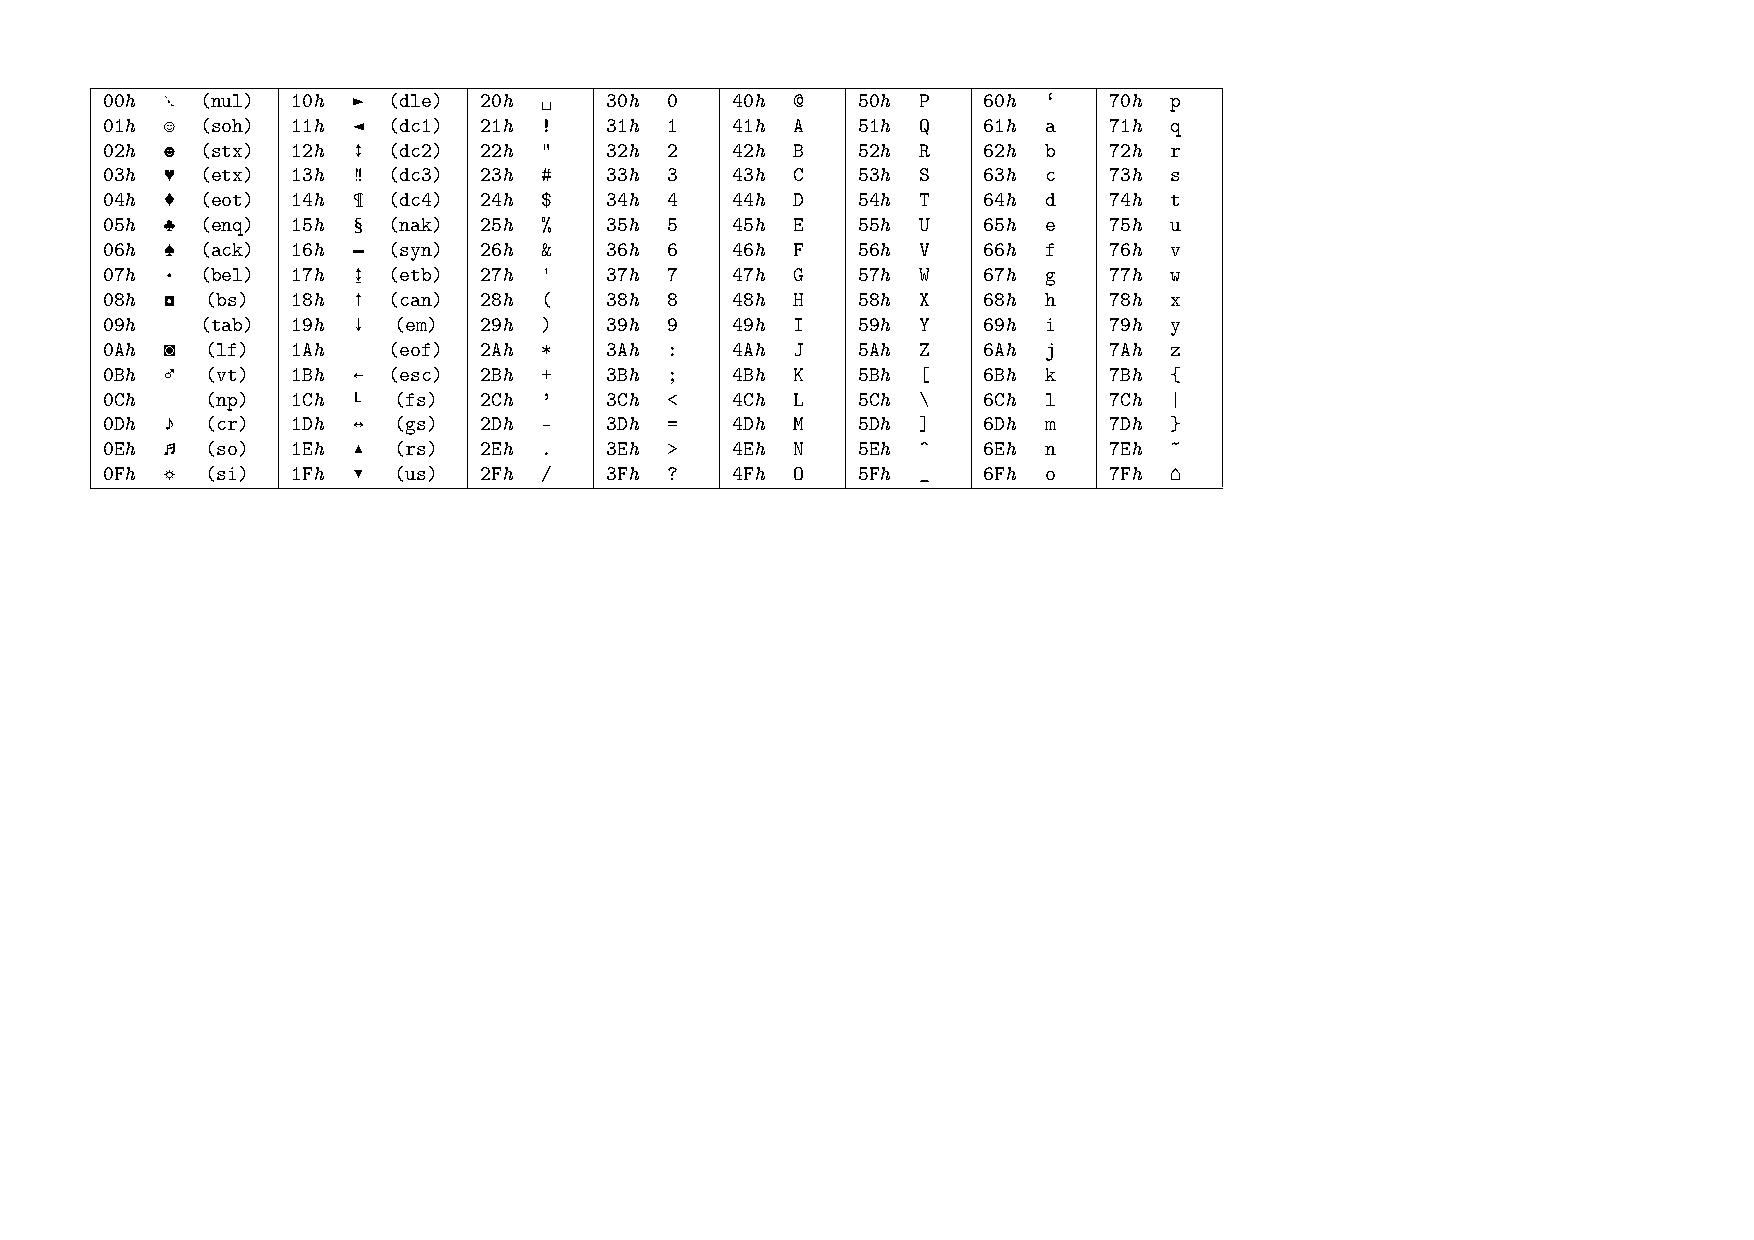
\includegraphics[width=0.85\textwidth]{figs/ascii.pdf}
	\centering
    \caption{La table ASCII}    
\end{figure}

Écrivez une fonction qui reçoit un \texttt{String} en argument (de taille 1 au minimum) et qui vérifie que les lettres dans le \texttt{String} sont toutes classées dans l'ordre de la table ASCII. Exemple:
\begin{scala}
progressive("ABCD") // Returns true
progressive("Aa") // Returns true
progressive("04Tu") // Returns true
progressive("ba") // Returns false
progressive("cZ") // Returns false
\end{scala}

\begin{solutionordottedlines}[\fill]
\begin{scala}
def progressive(s: String): Boolean = {
	var previous : Char = s.charAt(0)
	
	for(i <- 1 until s.length){
		if(previous > s.charAt(i)) {
			return false
		}
	
		previous = s.charAt(i)
	}
	return true
}	
\end{scala}
\end{solutionordottedlines}
\newpage

%%%%%%%%%%%%%%%%%%%
%% Double vowels
%%%%%%%%%%%%%%%%%%%
\part[4]
\subsection*{Double vowels}

Écrivez la fonction \texttt{doubleVowels} qui reçoit un \texttt{String} en argument et retourne un \texttt{String}. Le \texttt{string} retourné correspond au \texttt{String} reçu mais avec toutes les voyelles qui ont été doublées. Pour cet exercice les voyelles sont : \texttt{a}, \texttt{e}, \texttt{i}, \texttt{o}, \texttt{u}, \texttt{y}.

On considère par simplification que la chaîne en entrée est toujours en minuscule (donc pas besoin de gérer les lettres majuscules). Exemple:
\begin{scala} 
doubleVowels("hello") // Returns "heelloo"
doubleVowels("aabb") // Returns "aaaabb"
\end{scala}

\begin{solutionordottedlines}[14cm]
\begin{scala}	
def doubleVowels(s:String) : String = {
	var t: String = ""
	for (c <- s) {
		c match {
			case 'a'|'e'|'i'|'o'|'u'|'y' =>
				t = t + c + c
			case _ => 
				t += c
		}
	} 
	return t
}

// Other solution
def doubleVowels(s:String) : String = {
	var t: String = ""
	for (c <- s) {
		t += c match {
			case 'a'|'e'|'i'|'o'|'u'|'y' =>
				c + "" + c
			case _ => 
				c
		}
	} 
	return t
}
\end{scala}
\end{solutionordottedlines}

%%%%%%%%%%%%%%%%%%%
%% No triples 
%%%%%%%%%%%%%%%%%%%
\part[4]
\subsection*{No triples}
Le clavier de votre ordinateur est défectueux: quand vous tapez 2x de suite la même touche, il écrit 3x de suite le même caractère !

Écrivez la fonction \texttt{noTriples} qui corrige cette erreur dans la chaîne passée en argument. Notez que cette fonction n'interagit pas avec la console. Exemple:
\begin{scala}
"J'ai fait cettte illlusion" devient "J'ai fait cette illusion"
\end{scala}

\begin{solutionordottedlines}[15cm]
	\begin{scala}
	def noTriples(s:String) : String = {
		var t: String = ""
		var last: Char = 0
		var count: Int = 0
		
		for (c <- s) {
			if (last == c) {
				count += 1
			} else {
				count = 0
			}
			
			if (count != 2) {
				t += c
			}
		
			last = c
		}
		return t
	}	
	\end{scala}
\end{solutionordottedlines}
\end{parts}

\newpage

%%%%%%%%%%%%%%%%
%%% QUESTION %%%
%%%%%%%%%%%%%%%%%%%%%%%%%%%%%%%%%%%%%%%%
\titledquestion{Too fast, too furious}[5]
%%%%%%%%%%%%%%%%%%%%%%%%%%%%%%%%%%%%%%%%
Afin d'améliorer la sécurité sur les routes, les pandores valaisans vont installer un nouveau radar ultra moderne. Ce radar est en effet capable de calculer la vitesse moyenne entre deux points séparés par une certaine distance. 
 
Une infraction est alors constatée si la vitesse moyenne du véhicule est supérieure à la limitation de vitesse en cours. 

Écrivez les fonctions suivantes :

\begin{itemize}
	\item \texttt{def averageSpeed(timeOne : Double, timeTwo : Double, distance : Double)} re\-tour\-nant la vi\-tes\-se moy\-en\-ne entre les deux radars. Les deux paramètres de temps sont en secondes (remarque : seule la différence entre les deux temps est importante) et la valeur de retour doit être en km/h. La distance entre les deux radars est donnée en mètres.
	
	\item \texttt{isFaster}, un prédicat prenant comme arguments la vitesse du chauffeur et la limitation de vitesse et qui retourne si le chauffeur est en dehors des limitations.
	
	\item \texttt{getFineAmount(driverSpeed : Double, maxSpeed : Int)} retournant la valeur de l'amende que le chauffeur devra payer en cas d'infraction. 
\end{itemize}

Pour le dernier point, le montant de l'amende est calculé comme suit : 
 
\begin{itemize}
	\item une déduction de 5 \% doit être faite sur la vitesse mesurée. Arrondissez le résultat de cette déduction à l'unité (ex. 3.4 donne 3 et 3.6 donne 4).
    
    \item la facture s'élèvera à 60.- par tranche entamée de 10 km/h supérieurs à la limitation. Ainsi, le montant de l'amende doit être arrondi à la dizaine supérieure (23 km/h en trop vont être facturés comme 30 km/h).
\end{itemize}

\newpage
Votre solution:
\begin{solutionorbox}[\fill]
	\begin{scala}
		def averageSpeed(time1: Double, time2: Double, distance: Double) = (distance / (time2 - time1)) * 3.6
		def isFaster(speed: Double, maxSpeed: Double) = speed > maxSpeed
	  
		def getFineAmountSol1(speed: Double, maxSpeed: Int) = {
		  val realSpeed = ((speed - speed * 5.0 / 100.0) + 0.5).toInt
		  var price = 0
		  var s = realSpeed - maxSpeed
		  while (s > 0) {
			price += 60
			s -= 10
		  }
		  price
		}
	  
		// Other solution
		def getFineAmountSol2(speed: Double, maxSpeed: Int) = {
		  val realSpeed = ((speed - speed * 5.0 / 100.0) + 0.5).toInt
		  val diff = realSpeed - maxSpeed
	  
		  if (diff % 10 == 0)
			diff / 10 * 60
		  else if (diff > 0)
			((diff / 10) + 1) * 60
		  else 0
		}
	\end{scala}
\end{solutionorbox}

\newpage
\lastPage 

\end{questions}
\end{document}

%%%% This is the end, beautiful friend the end.